
In the given  problem
\begin{align}
\vec{A}_1= \myvec{-1\\-1\\-1}, \vec{m}_1=\myvec{7 \\ -6 \\1},
\vec{A}_2= \myvec{3\\5\\7}, \vec{m}_2 =\myvec{1 \\ -2 \\1}.
\end{align}
The lines will intersect if
\begin{align}
\myvec{-1\\-1\\-1} + \lambda_1\myvec{7 \\ -6 \\1}
= \myvec{3\\5\\7} + \lambda_2\myvec{1 \\ -2 \\1}
\\
\implies \lambda_1\myvec{7 \\ -6 \\1} - \lambda_2\myvec{1 \\ -2 \\1} &= \myvec{3\\5\\7}-\myvec{-1\\-1\\-1}  
\\
\implies \myvec{7 & 1 \\ -6 & -2 \\ 1 & 1}\myvec{\lambda_1\\ \lambda_2} = \myvec{4\\6\\8}\label{sep/2/22/condition}
\end{align}
Row reducing the augmented matrix,
\begin{align}
\myvec{
7 & 1 & 4 
\\
-6 & -2 & 6
\\
1 & 1 & 8
}
\xleftrightarrow[]{R_3\leftrightarrow R_1}
\myvec{
1 & 1 & 8
\\
-6 & -2 & 6
\\
7 & 1 & 4
}
\\
\xleftrightarrow[]{\substack{R_2= 6R_1+R_2\\R_3 = -7R_1+R_3}}
\myvec{
1 & 1 & 8
\\
0 & 4 & 54
\\
0 & -6 & -52
}
\xleftrightarrow[]{R_2= \frac{R_2}{4}}
\myvec{
1 & 1 & 8
\\
0 & 1 & \frac{27}{2}
\\
0 & -6 & -52
}
\\
\xleftrightarrow[]{R_3=6R_2+R_3}
\myvec{
1 & 1 & 8
\\
0 & 1 & \frac{27}{2}
\\
0 & 0 & 29
}
\end{align}
The above matrix has $rank = 3$.  Hence, the lines do not intersect.  Note that the lines are not parallel but they  lie on parallel planes.  Such lines are known as {\em skew} lines as can be seen in Fig \ref{sep/2/22/skew_lines}.\\
$\therefore$ The distance between given two lines is (using  equation \eqref{sep/2/22/condition})
\begin{align}
\norm{\myvec{7 & 1 \\ -6 & -2 \\ 1 & 1}\myvec{\lambda_1\\ \lambda_2} - \myvec{4\\6\\8}}
\end{align}
We know that, the minimizer of $\norm{\vec{A}\vec{x} - \vec{B}}$ is given by the solution to the normal equations $\vec{A}^{T}\vec{A}\vec{x} = \vec{A}^{T}\vec{B}$. Since
\begin{align}
\myvec{7 & 1 \\ -6 & -2 \\ 1 & 1}^{T}\myvec{7 & 1 \\ -6 & -2 \\ 1 & 1} &= \myvec{86 & 20 \\ 20 & 6}\\
\myvec{7 & 1 \\ -6 & -2 \\ 1 & 1}^{T}\myvec{4\\6\\8} &= \myvec{0 \\ 0}
\end{align}
the normal equations give us the following system of equations
\begin{align}
\myvec{86 & 20 \\ 20 & 6}\myvec{\lambda_1\\ \lambda_2} = \myvec{0 \\ 0}
\end{align}
whose solution is $\myvec{\lambda_1\\ \lambda_2} = \myvec{0\\ 0}$. The minimum distance between this two lines is, thus,
\begin{align}
\norm{\myvec{7 & 1 \\ -6 & -2 \\ 1 & 1}\myvec{0 \\ 0} - \myvec{4\\6\\8}} &= \norm{\myvec{4\\6\\8}}\\
																		 &= \sqrt{116}
\end{align}
\begin{figure}[!ht]
\centering 
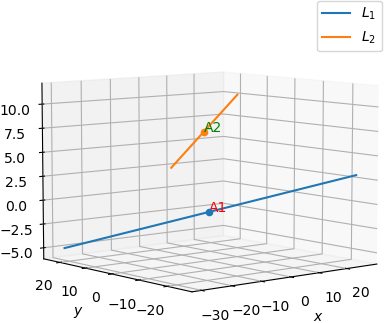
\includegraphics[width=\columnwidth]{solutions/sep/2/22/Figures/plot.png}
\caption{plot of lines}
\label{sep/2/22/skew_lines}
\end{figure}
